\subsection{电解溶剂法}
电解溶剂法是从溶液中生长晶体的一种独特的方法。其原理基于用电解法分解溶剂,以除去溶剂,使溶液处于过饱和状态。显然这种方法只能应用于溶剂可以被电解而其产物很容易自溶液中移去(如气体)的体系。同时还要求所培养的晶体在溶液中能导电而又不被电解。因此,这种方法特别适用于一些稳定的离子晶体的水溶液体系。

电解溶剂法的一半装置如图3.25所示。育晶器中装有铂电极,也起电解槽的作用,当通以稳定的直流电,溶剂就被电解,其速度由电流密度控制。溶液要搅拌以免产生浓差极化。溶液表面用流动液层(如邻二甲苯)覆盖以防溶剂蒸发,电解的产物从冷凝器中排除,在生长过程中,溶液pH应保持稳定。

\begin{figure}[h]
 \centering
 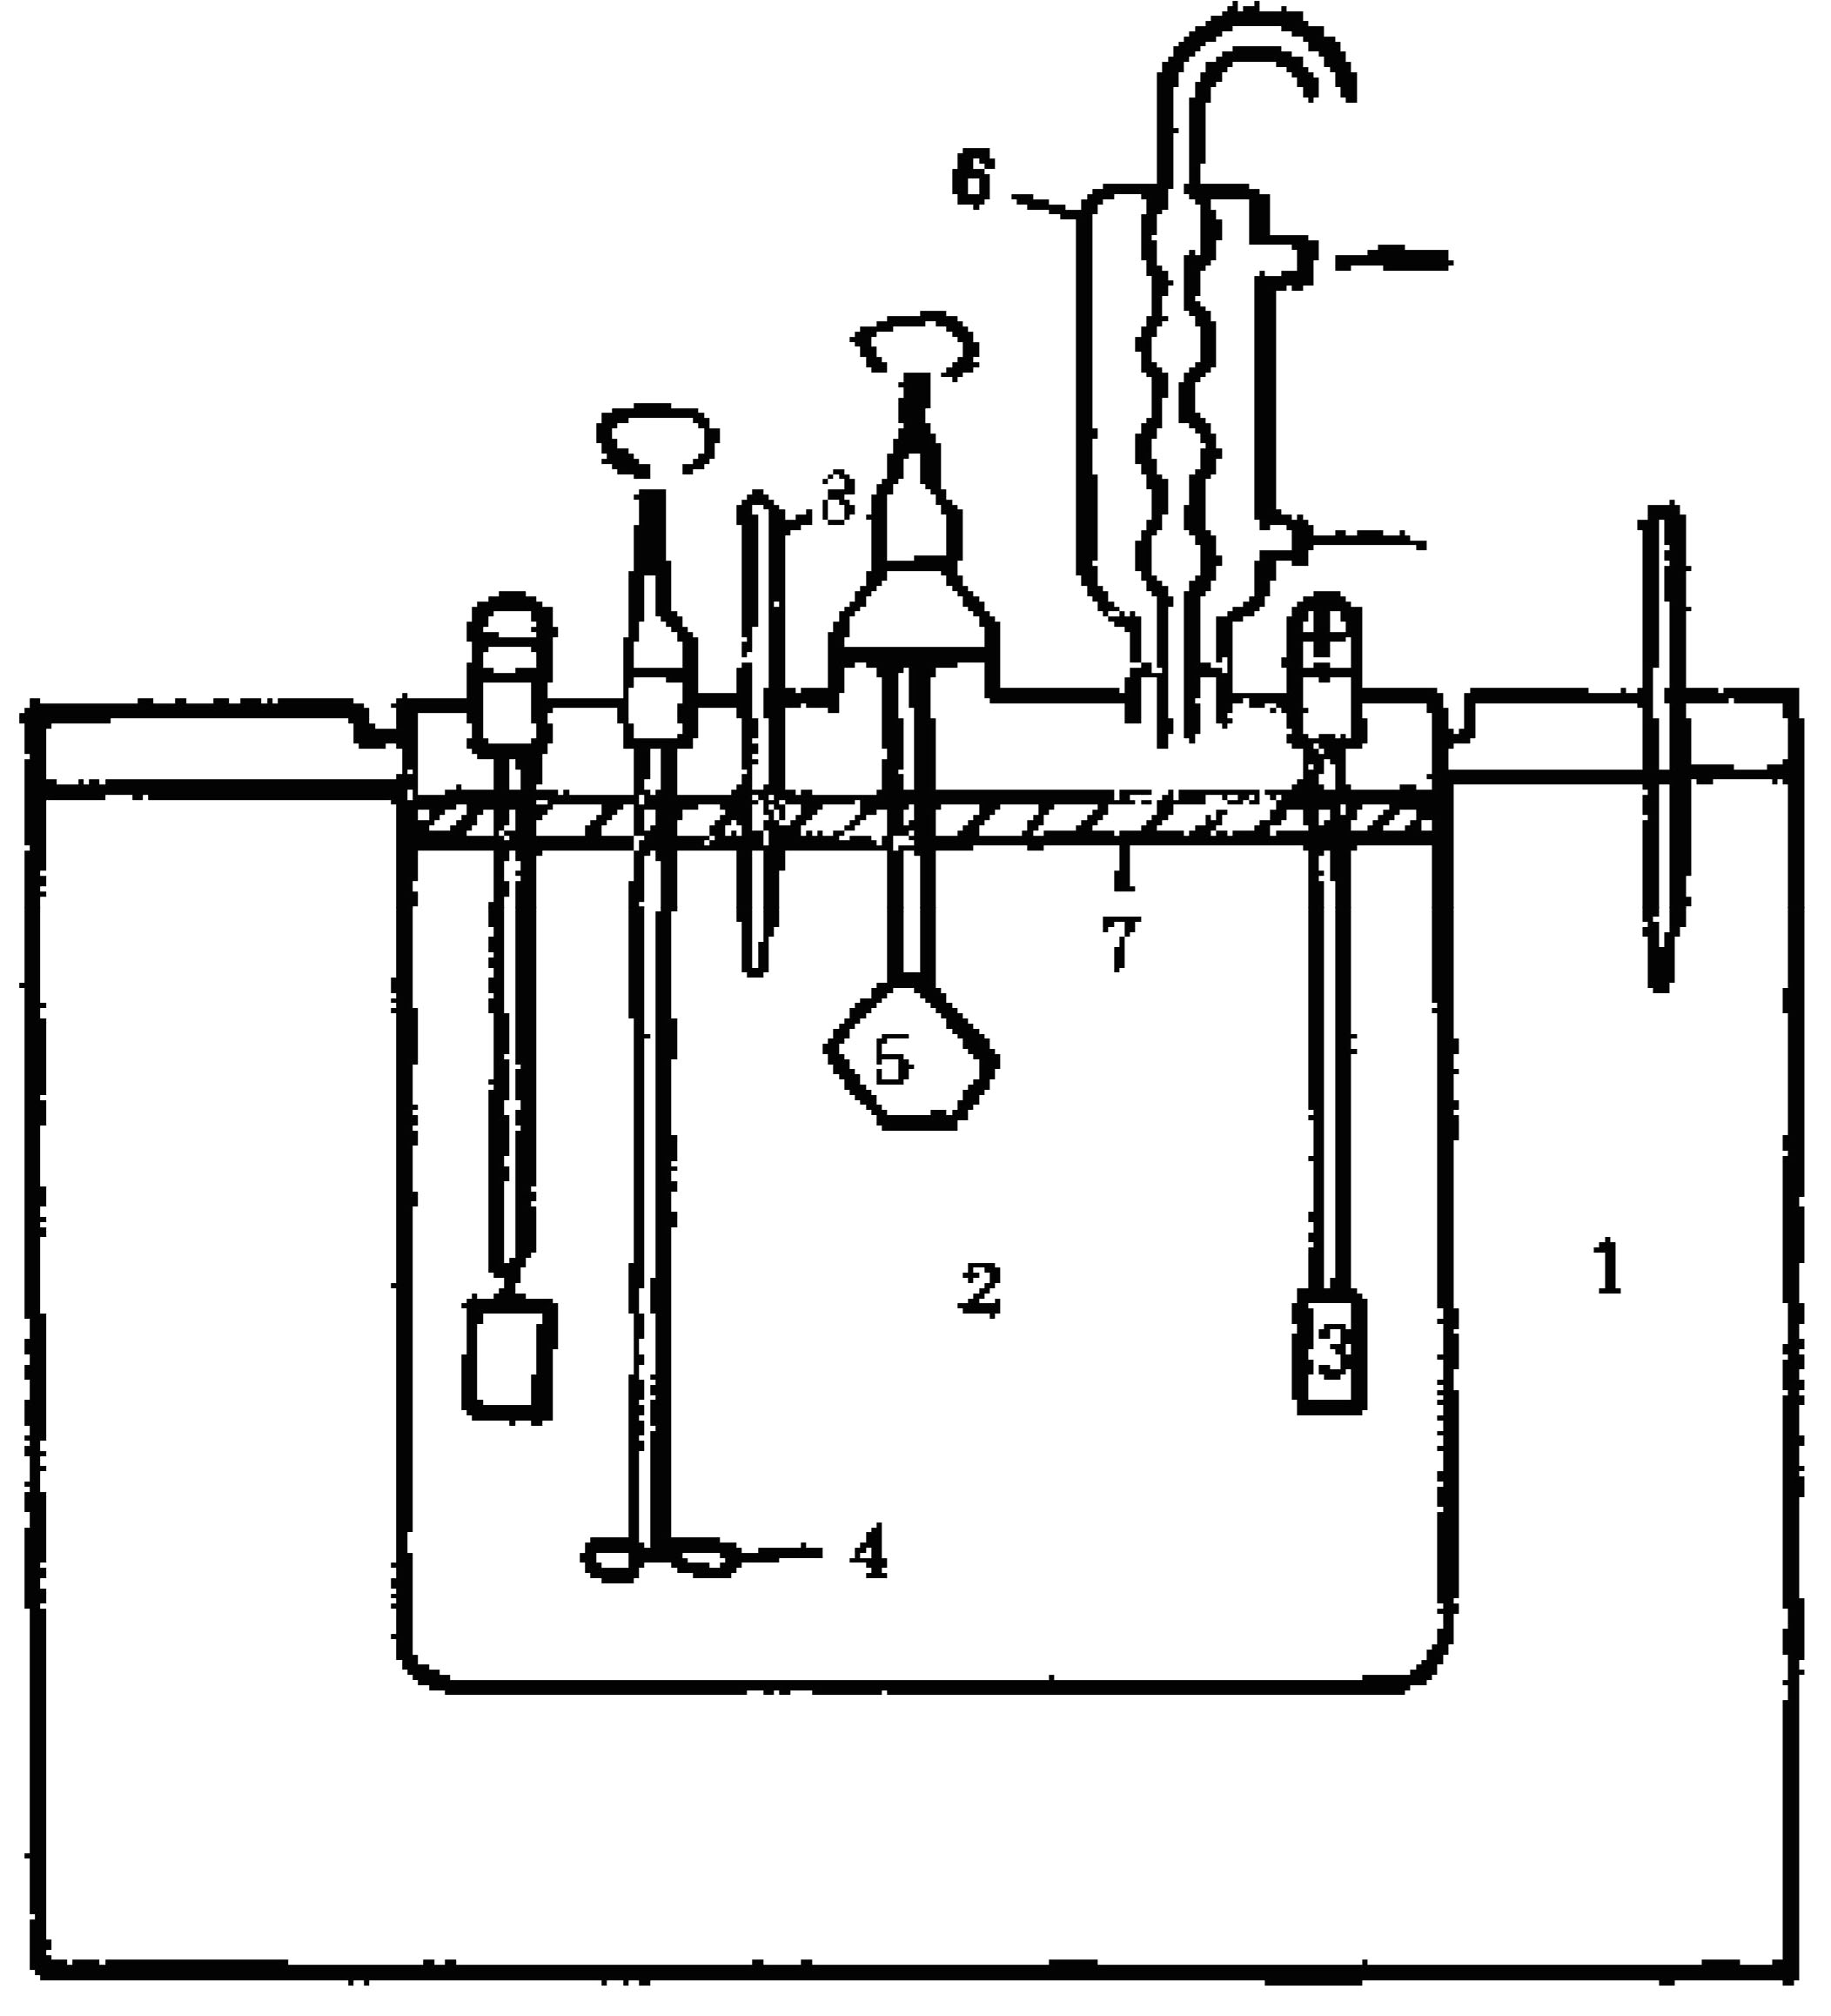
\includegraphics[width=0.8\textwidth]{fig/cp03/img3.25.jpg}
 \caption{电解溶剂法生长晶体装置图。}
\end{figure}

和流动法和蒸发法一样,用电解溶剂法生长晶体也是恒温下进行的。由于过饱和度使用直流电准确控制的,因此和生长温度关系不大,也可在室温下进行(这一点比蒸发法优越,因为温度较低时,蒸发量小,难以控制),也不需要知道溶解度曲线的情况。所以这种方法既适用于溶解度温度系数比较小的晶体,也适用于生长有数种晶相存在,而每种晶相仅在一定温度范围内才能稳定存在的晶体。

用电解溶剂法来生长KDP型(特别是DKDP晶体)获得了满意的结果。因为溶液中存在的常导致这些晶体柱面楔化的一些金属杂质离子(如Fe$^{3+}$,Al$^{3+}$,Cr$^{3+}$等)可以在电解过程中除去,从而消除这些杂质的有害影响。对DKDP晶体可以在低于其转变点的温度下生长,以防止单斜相的干扰,由于分解H$_2$O所需的能量比分解D$_2$O的要低,溶液中的H$_2$O在电解过程中比较容易除去。溶液在生长过程中可以保持较高的氘化程度。图3.26示出在普通转晶育晶器(图3.18)基础上改装的电解溶剂法生长这一类晶体的装置。阳极置于育晶器底部,为使电流均匀通过溶液,在溶液上方安置了两个电极,阴极放在喇叭形口的塑料管内,口上用尼龙网覆盖,使在阴极上产生的氢气引入通风良好的空间,防止其重新进入溶液。在阳极上产生的氧气进入育晶器中溶液上方的空间,保持正压,它投注于减少大气中的水汽和溶液中的氘发生交换而降低其含氘量。由于电解交流也会产生热量,因此也可以不使用底部加热器,而是将交流电直接通过电极加热,使用交、直流并用的加热—电解联合控制装置。晶体在溶液中转动以使溶液浓度均匀。由于溶液是强缓冲溶液,所以电解过程中溶液pH变化不大。

\begin{figure}[h]
 \centering
 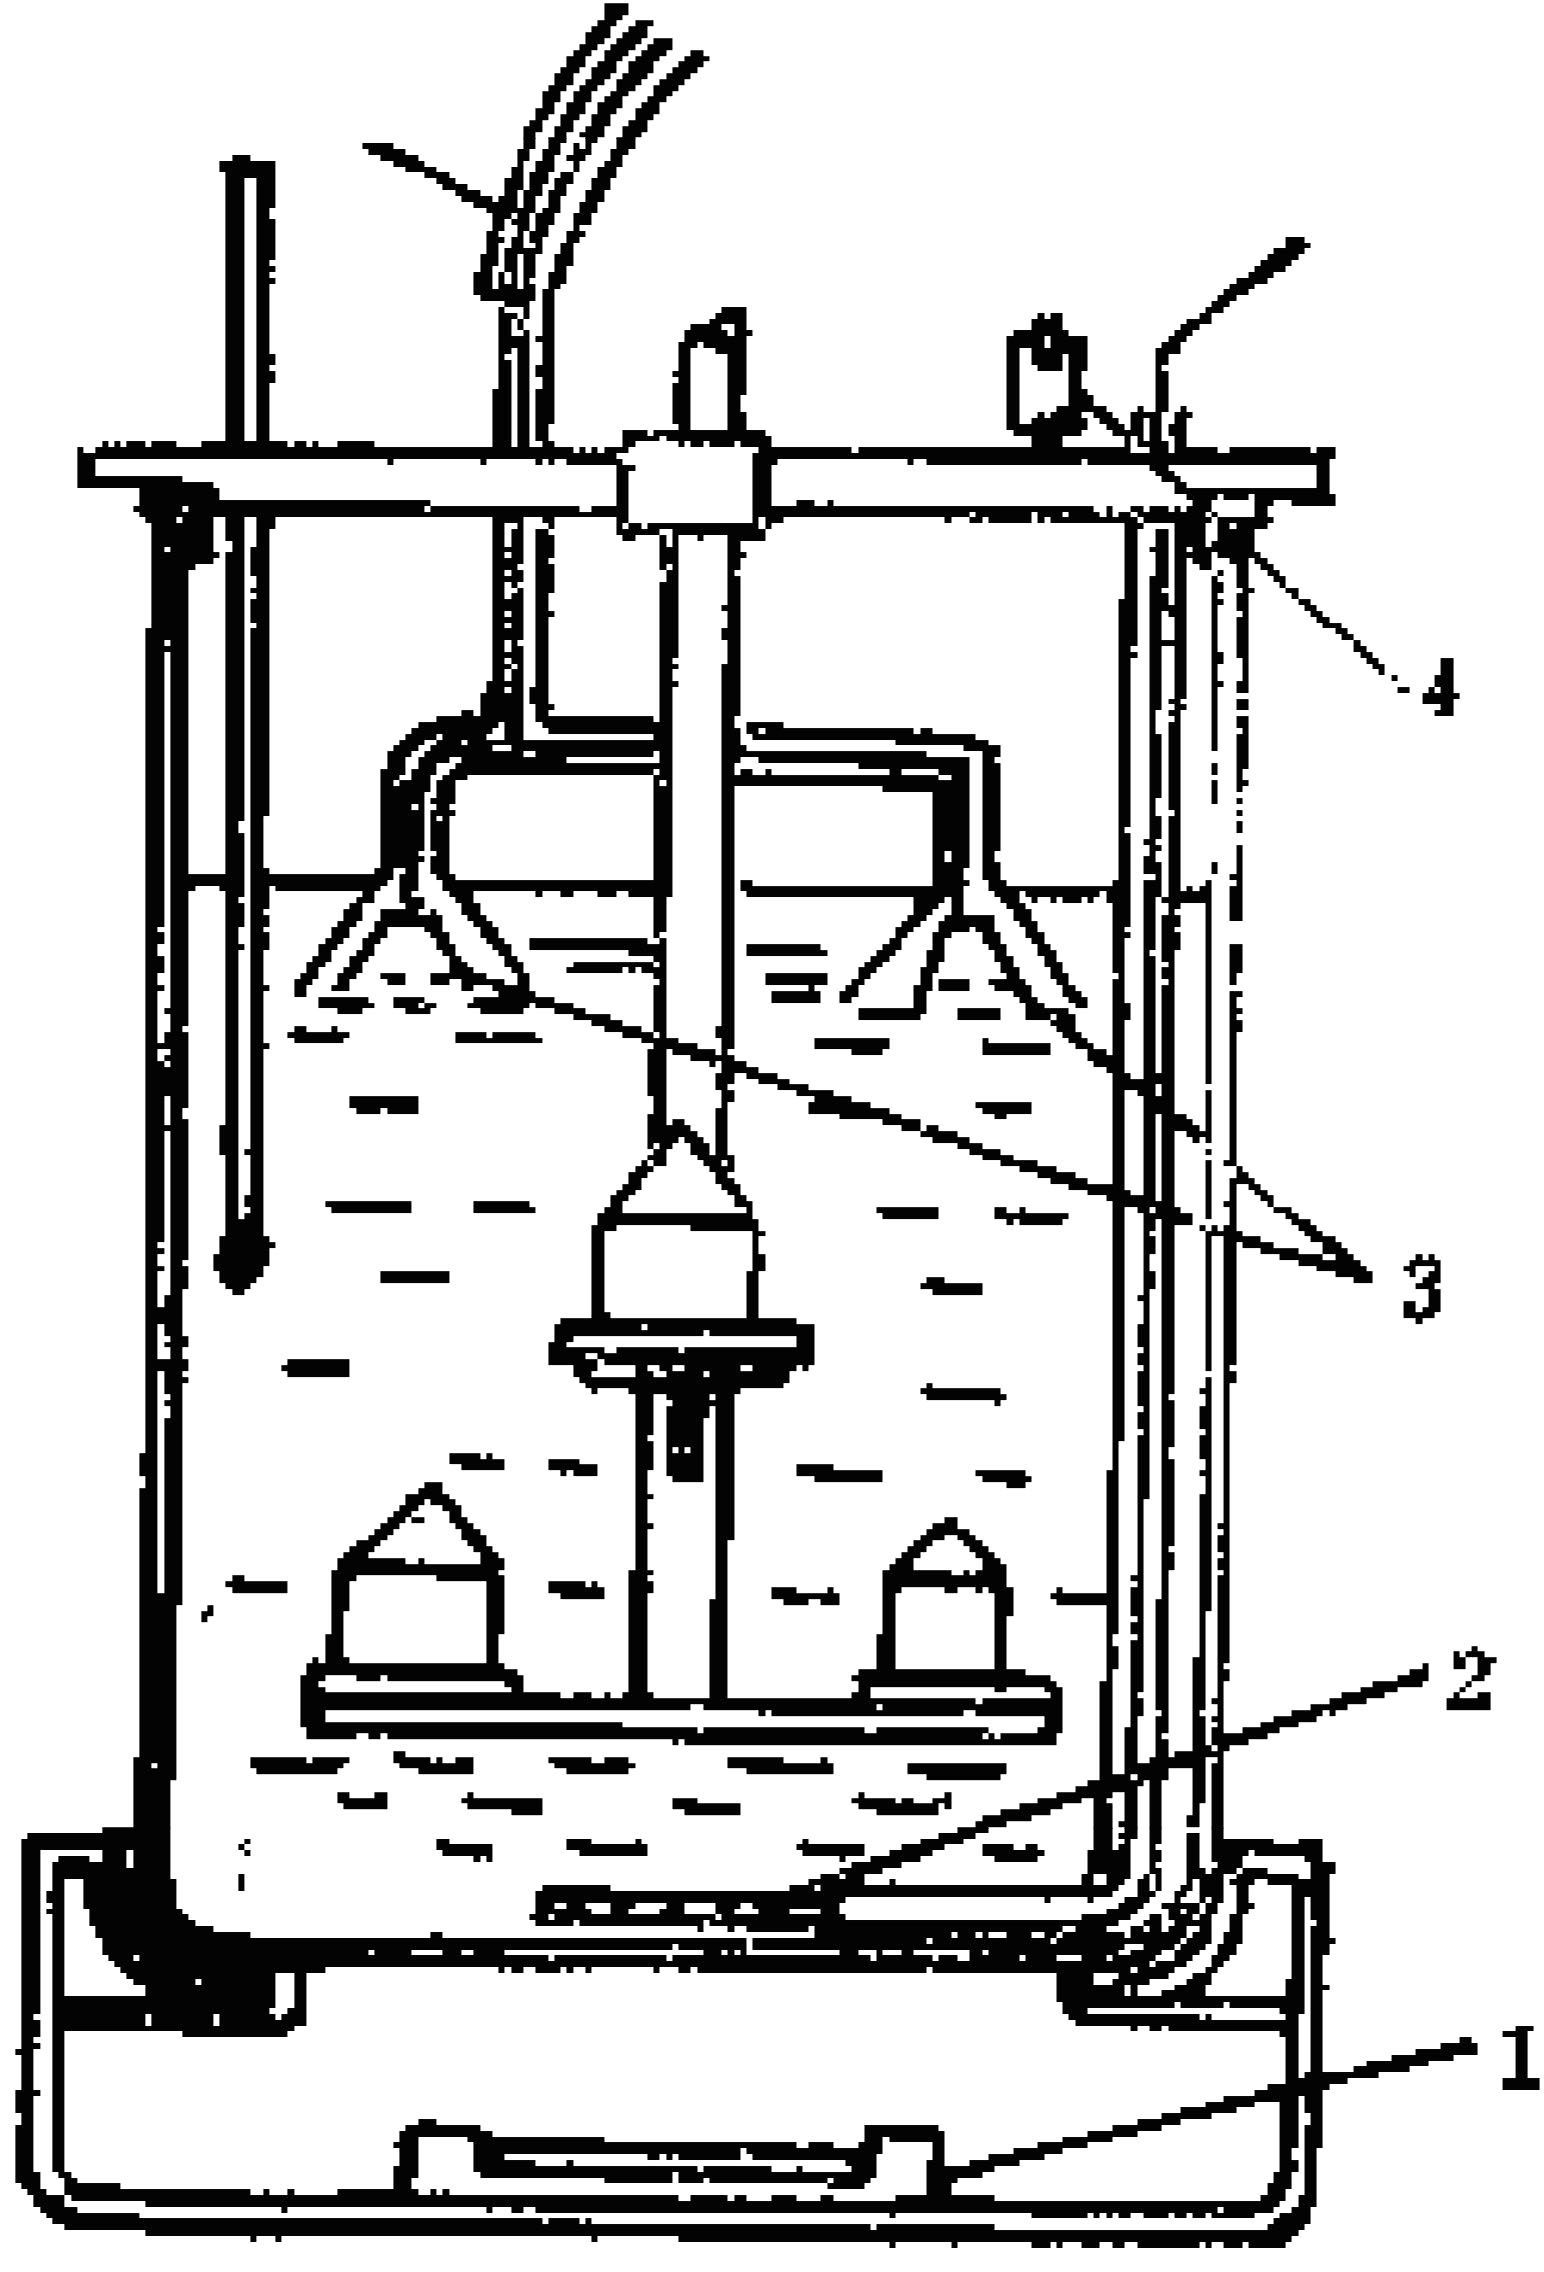
\includegraphics[width=0.8\textwidth]{fig/cp03/img3.26.jpg}
 \caption{由通常转晶育晶器改装的电解溶剂育晶装置。}
\end{figure}

对于从重水溶液中生长高质量的KDP型晶体,电解溶剂法是一种有前途的方法。

除了上述四种从水溶液中生长晶体的方法外,还有凝胶法,有机溶剂法等,这些内容将在下面独立的章节中进行论述。

上述的从溶液中生长晶体的各种方法中,以降温法、蒸发法、流动法最为常用,大部分水溶性晶体都是用这些方法培养的。表3.9列出了从溶液中生长的一些晶体的单晶培养和一般的结晶方法。

(表3.9  从溶液中生长的一些重要晶体)

